%(BEGIN_QUESTION)
% Copyright 2006, Tony R. Kuphaldt, released under the Creative Commons Attribution License (v 1.0)
% This means you may do almost anything with this work of mine, so long as you give me proper credit

Et fritt bevegelig stempel inne i en hydraulikksylinder har 1000 PSI fluidtrykk på den ene siden og 850 PSI på den andre siden. Stempelet har diameter 2.75 tommer. Hvor stor kraft virker på stempelet med disse trykkene?

$$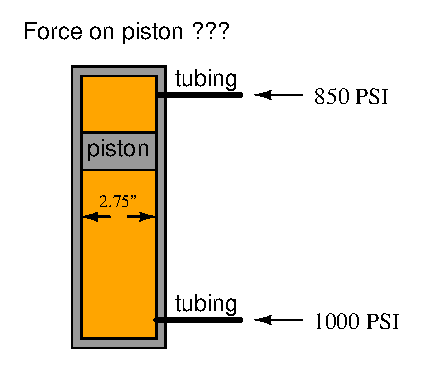
\includegraphics[width=15.5cm]{i00155x01.eps}$$

\underbar{file i00155}
%(END_QUESTION)





%(BEGIN_ANSWER)

Netto stempelkraft = 890.936 pund.

\vskip 10pt

I dette tilfellet virker to trykk mot hverandre: 850 PSI presser nedover, mens 1000 PSI presser oppover. Resultatet (differansetrykket) er 150 PSI (1000 - 850). Dette er trykkverdien som brukes i sluttberegningen av kraft.

%(END_ANSWER)





%(BEGIN_NOTES)

%INDEX% Physics, fluids: pressure, force, and area

%(END_NOTES)
